\section{Objectives}

Rebuild Fig. 27.1(a)--(d) from handout PDF pages 111--114, examining two-phase skew, fixed inputs, and output glitches while distinguishing logical NORA race conditions from analog integrity.

\section{Handout requirements and test mapping}

\begin{center}
\small
\setlength{\tabcolsep}{4pt}
\begin{tabular}{p{.42\linewidth}p{.29\linewidth}p{.18\linewidth}}
\toprule
Requirement & Deck prefix and conditions & Status \\
\midrule
Step: four circuits with/without skew & 01; 0, +0.5, -0.5 ns & Independent full circuits \\
Q1: input fixed at 0 and 1 & 01; each skew repeated & 9 cases total \\
Q2: compare safety of b/c/d & Settled samples + full waveform & Glitches measured/discussed \\
\bottomrule
\end{tabular}
\end{center}

\section{Topology and NORA conditions}

Each circuit independently uses an initial clocked inverter, a static inverter, and an N-dynamic NAND with its other input fixed at 1. Circuit (a) inserts one static inverter between the N-dynamic gate and final latch; (b) uses a P-dynamic stage followed by a clocked inverter; (c) uses two clocked inverters; (d) uses a clocked inverter followed by a static inverter. Independent upstream copies avoid unequal fanout caused by sharing nodes.

Safe NORA composition must respect evaluation direction and inversion parity: dynamic/static inversion counts and latch placement within each phase section must follow the handout rules, preventing precharge transitions from propagating as data to the next storage point. This is a logical race condition; it does not automatically eliminate charge sharing, clock feedthrough, or analog glitches from finite edges.

\section{Simulation setup and interpretation}

The supplied encrypted MOS model is evaluated at a baseline supply of 1.0 V and 25\,$^\circ$C. The 1.0 V value is a teaching condition, not a verified voltage rating. These results do not reproduce the handout's original process or supply conditions. Unless stated in the deck, $W_n/W_p/L=0.6/1.8/0.25\,\mu\mathrm m$, bulks are tied to their corresponding rails, and output load is 5 fF. Transmission-gate and weak-feedback dimensions are specified explicitly in each deck.

PrimeSim HSPICE S-2021.09 win64 was used with \texttt{RUNLVL=6}, \texttt{ACCURATE}, and \texttt{WARNLIMIT=100}. Every baseline and \texttt{.alter} analysis concluded without errors or failed measurements. The simulator still reports suppressed warnings associated with encrypted blocks; this does not establish that the model is warning-free or that those warnings are harmless. The \texttt{.tran} print interval is not a fixed integration step: the solver uses adaptive timesteps. A finite sweep is not a complete process qualification.

Unless stated otherwise, the declared functional diagnostic uses $V\leq0.2$ V for low and $V\geq0.8$ V for high. These are report-level interpretation thresholds, not numerical handout requirements or extracted receiver noise margins. Correct samples do not exclude glitches between samples. Figures are redrawn from actual simulation data; \texttt{results/} contains per-case waveforms, measurements, and derived comparison CSV files.

Public decks omit model loading paths; model configuration is added only to local execution copies. The model itself is not distributed. The first two filename digits identify the deck numbers used below. Every deck is standalone.

\section{Results}

The period is 4 ns and both phase-source edges are 0.2 ns. The complementary phase is independently shifted by 0, +0.5, or -0.5 ns. Dynamic data and fixed 0/1 inputs each repeat all three skews, giving nine analyses. All circuits match the inverted data at the six settled samples at 10.6, 14.6, 18.6, 22.6, 26.6, and 30.6 ns, but full waveforms contain substantial erroneous pulses.

\begin{figure}[htbp]
\centering
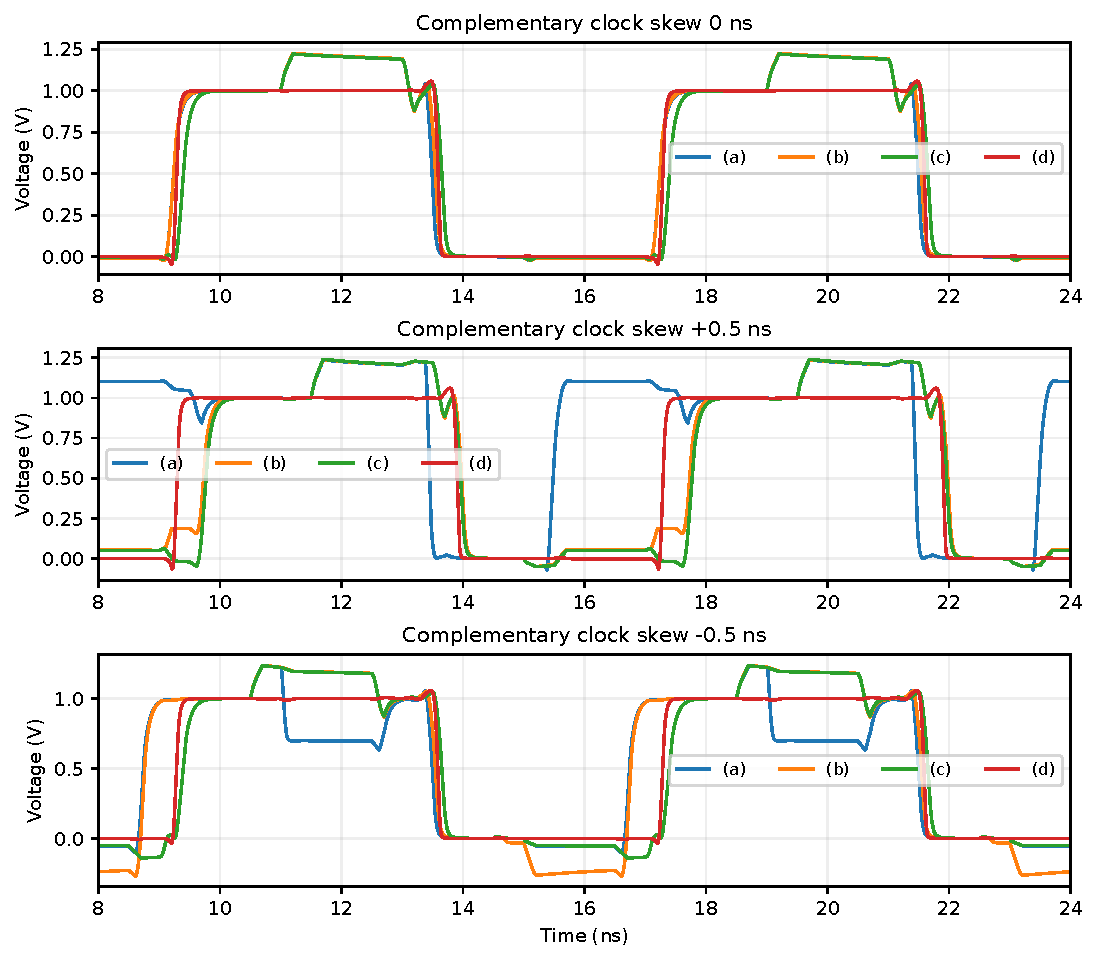
\includegraphics[width=.96\linewidth]{figures/four_topologies.pdf}
\caption{Four topologies with changing data; fixed-time samples do not cover the entire hold interval.}
\end{figure}

\begin{center}
\small
\setlength{\tabcolsep}{4pt}
\begin{tabular}{lrrrr}
\toprule
Skew (ns) & (a) maximum (V) & (b) maximum (V) & (c) maximum (V) & (d) maximum (V) \\
\midrule
0 & 0.92728 & 0.95661 & 0.11694 & 0.42357 \\
0.5 & 1.10902 & 0.86663 & 0.14575 & 0.97954 \\
-0.5 & 1.05679 & 1.04569 & 0.17798 & 0.51725 \\
\bottomrule
\end{tabular}
\end{center}

\begin{figure}[htbp]
\centering
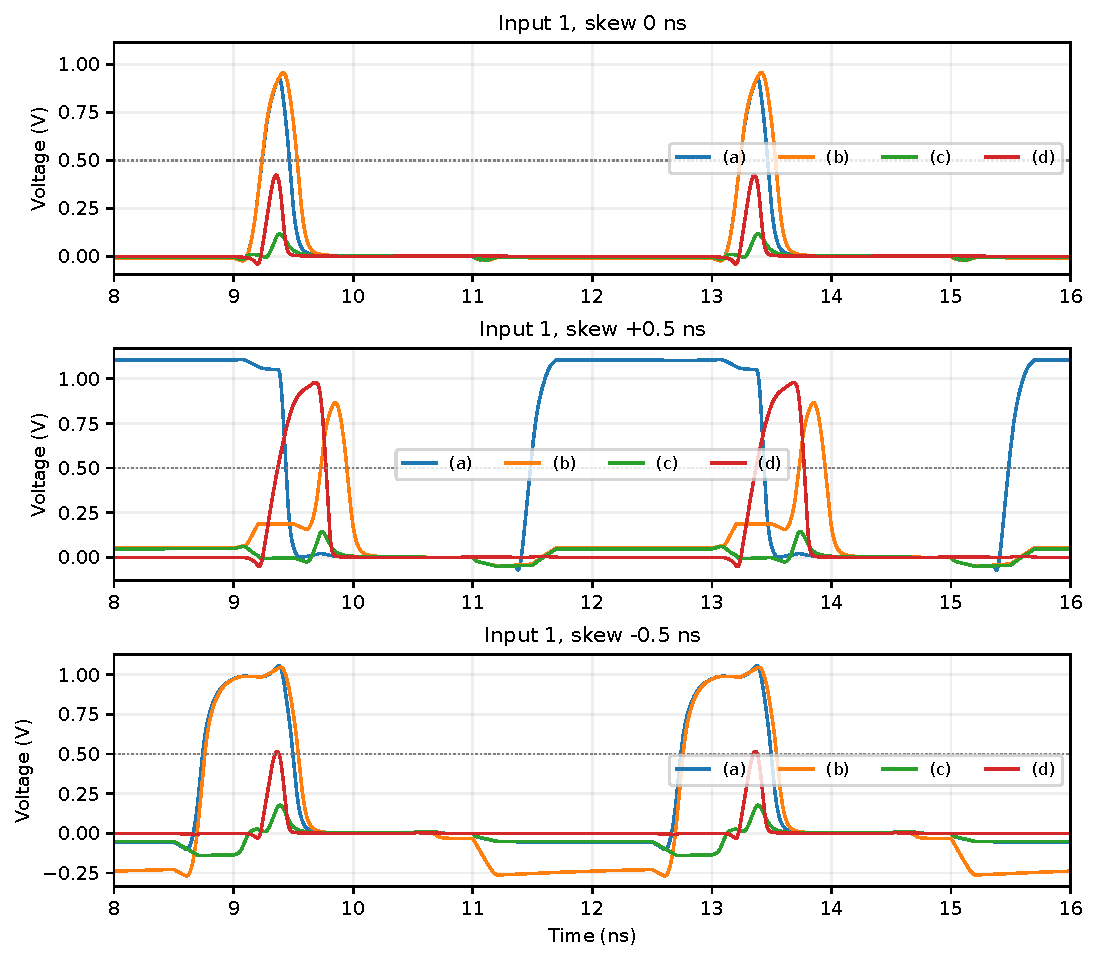
\includegraphics[width=.96\linewidth]{figures/fixed_input_glitches.pdf}
\caption{With input fixed at 1, ideal output is 0; the dotted line marks 0.5 V for observation.}
\end{figure}

With input fixed at 1, circuit (a) errors are not restricted to data transitions; positive skew produces a wider erroneous high interval. Circuit (b) also has pulses crossing 0.5 V, and (d) reaches 0.97954 V at +0.5 ns. Circuit (c) peaks at no more than 0.17798 V across these skews and holds low best in this test. With input fixed at 0, (a)/(b)/(c) minima are approximately 0.87 V with feedthrough maxima around 1.22--1.24 V; circuit (d) keeps its high level closer to the rail.

\section{Discussion, differences, and unverified scope}

Q1: fixed-input testing excludes a data-transition-only explanation; precharge, clock coupling, and transparency windows can cause errors by themselves. Q2: circuit (c) holds low most reliably under these conditions, but one model, load, and three skews cannot establish unconditional safety. The glitches in (b)/(d) cannot all be labeled logical race from output traces alone: dynamic-node charge and subsequent amplification can look similar. Internal-node CSV data is retained for mechanism tracing. Six correct settled samples are not a full-window race-free acceptance. If a design requires no threshold crossing throughout the hold window, (a)/(b)/(d) have not met it here; the handout topologies are preserved to expose that difference.
